\chapter*{}

\section{Brolasi}

\begin{figure}[h!]
    \centering
    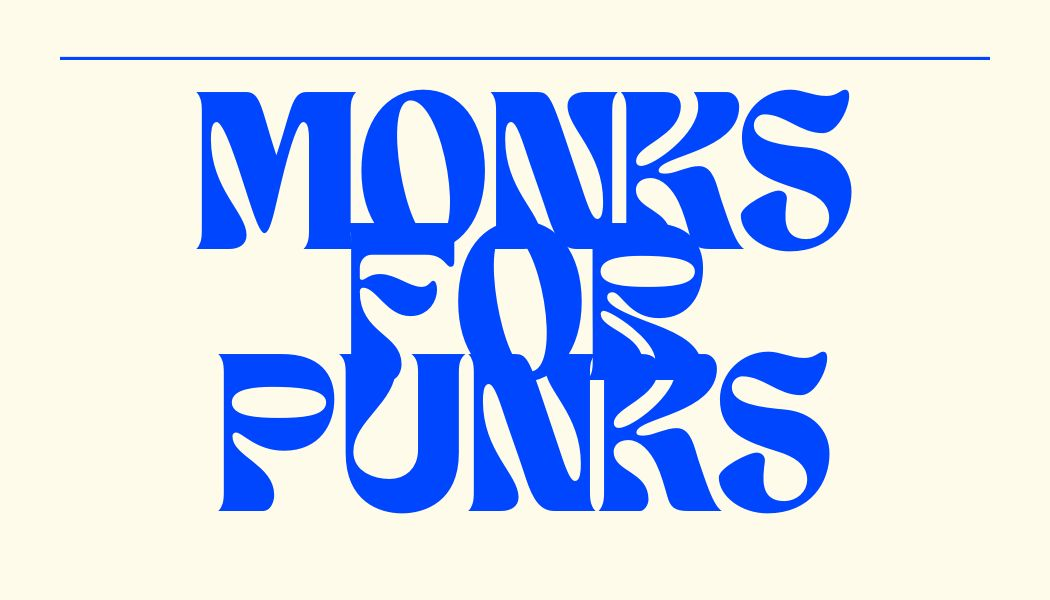
\includegraphics[width=0.5\textwidth]{images/Monks_For_Punks_Front.jpg}
    \label{fig:Monks_For_Punks}
\end{figure}

\subsection {Cantrips}
\DndSpellHeader%
  {\textbf{Force Blast}}
  {Evocation Cantrip}
  {1 action}
  {180 feet}
  {V, S}
  {Instantaneous}
  %{\textbf{Attack/Save}: WIS 13}\\\
  
You unleash a bolt of mystical power at a creature or an object within range. Make a ranged spell attack against the target. On a hit, the target takes 1d8 Force damage.

{\textbf{Cantrip Upgrade.}} This damage increases by 1d8 when you reach levels 5 (2d8), 11 (3d8), and 17 (4d8).


\DndSpellHeader%
{\textbf{Light}}
{Evocation Cantrip}
{1 action}
{Touch}
{V, M (a firefly or phosphorescent moss)}
{1 Hour}
%{\textbf{Attack/Save}: WIS 13}\\\

You touch one Large or smaller object that isn’t being worn or carried by someone else. Until the spell ends, the object sheds Bright Light in a 20-foot radius and Dim Light for an additional 20 feet. The light can be colored as you like.

Covering the object with something opaque blocks the light. The spell ends if you cast it again.


\DndSpellHeader%
{\textbf{Spare the Dying}}
{Necromancy Cantrip}
{1 action}
{15 ft}
{V, S}
{Instantaneous}
%{\textbf{Attack/Save}: WIS 13}\\\

Choose a creature within range that has 0 Hit Points and isn’t dead. The creature becomes Stable.
\textbf{Cantrip Upgrade.} The range doubles when you reach levels 5 (30 feet), 11 (60 feet), and 17 (120 feet).



\DndSpellHeader%
{\textbf{Toll of the Dead}}
{Necromancy Cantrip}
{1 action}
{60 ft}
{V, S}
{Instantaneous}
{\textbf{Attack/Save}: WIS 14}\\\

You point at one creature you can see within range, and the single chime of a dolorous bell is audible within 10 feet of the target. The target must succeed on a Wisdom saving throw or take 1d8 Necrotic damage. If the target is missing any of its Hit Points, it instead takes 1d12 Necrotic damage.
\textbf{Cantrip Upgrade.} The damage increases by one die when you reach levels 5 (2d8 or 2d12), 11 (3d8 or 3d12), and 17 (4d8 or 4d12).


\subsection{Class Features}
\begingroup
\DndSetThemeColor[PhbMauve]

\begin{DndComment}{Lay Hands}
	Your blessed touch can heal wounds. You have a pool of healing power that replenishes when you finish a Long Rest. With that pool, you can restore a total number of Hit Points equal to five times your Paladin level.
	As a Bonus Action, you can touch a creature (which could be yourself) and draw power from the pool of healing to restore a number of Hit Points to that creature, up to the maximum amount remaining in the pool.
	You can also expend 5 Hit Points from the pool of healing power to remove the Poisoned condition from the creature; those points do not also restore Hit Points to the creature.
\end{DndComment}

\begin{DndComment}{Spellcasting}
	You have learned to cast spells through prayer and meditation.
	
	Spell Slots. The Paladin Features table shows how many spell slots you have to cast your level 1+ spells. You regain all expended slots when you finish a Long Rest.
	
	Prepared Spells of Level 1+. You prepare the list of level 1+ spells that are available for you to cast with this feature. To start, choose two level 1 Paladin spells.
	
	The number of spells on your list increases as you gain Paladin levels, as shown in the Prepared Spells column of the Paladin Features table. Whenever that number increases, choose additional Paladin spells until the number of spells on your list matches the number in the Paladin Features table. The chosen spells must be of a level for which you have spell slots. For example, if you’re a level 5 Paladin, your list of prepared spells can include six Paladin spells of level 1 or 2 in any combination.
	
	If another Paladin feature gives you spells that you always have prepared, those spells don’t count against the number of spells you can prepare with this feature, but those spells otherwise count as Paladin spells for you.
	
	Changing Your Prepared Spells. Whenever you finish a Long Rest, you can replace one spell on your list with another Paladin spell for which you have spell slots.
	
	Spellcasting Ability. Charisma is your spellcasting ability for your Paladin spells.
	
	Spellcasting Focus. You can use a Holy Symbol as a Spellcasting Focus for your Paladin spells.
\end{DndComment}

\begin{DndComment}{Weapon Mastery}
	Your training with weapons allows you to use the mastery properties of two kinds of weapons of your choice with which you have proficiency.
	
	Whenever you finish a Long Rest, you can change the kinds of weapons you chose.
	
	\textbf{Quarterstaff (Topple).} Your training with weapons allows you to use the mastery property of Quarterstaffs:
	
	\textbf{Topple:} If you hit a creature with a Quarterstaff, you can force the creature to make a Constitution saving throw (DC 8 plus the ability modifier used to make the attack roll and your Proficiency Bonus). On a failed save, the creature has the Prone condition.
	
	\textbf{Longsword (Sap)} Your training with weapons allows you to use the mastery property of Longswords:
	
	\textbf{Sap:} If you hit a creature with a Longsword, that creature has Disadvantage on its next attack roll before the start of your next turn.
	
	\textbf{Topple (Quarterstaff):} 1 Action
	
	\textbf{Sap (Longsword):} 1 Action

\end{DndComment}


\begin{DndComment}{Channel Divinity}
	You can channel divine energy directly from the Outer Planes, using it to fuel magical effects. You start with one such effect: Divine Sense, which is described below. Other Paladin features give additional Channel Divinity effect options. Each time you use this class’s Channel Divinity, you choose which effect from this class to create.
	
	You can use this class’s Channel Divinity twice. You regain one of its expended uses when you finish a Short Rest, and you regain all expended uses when you finish a Long Rest. You gain an additional use when you reach Paladin level 11.
	
	If a Channel Divinity effect requires a saving throw, the DC equals the spell save DC from this class’s Spellcasting feature.
	
	\textbf{Divine Sense:} As a Bonus Action, you can open your awareness to detect Celestials, Fiends, and Undead. For the next 10 minutes or until you have the Incapacitated condition, you know the location of any creature of those types within 60 feet of yourself, and you know its creature type. Within the same radius, you also detect the presence of any place or object that has been consecrated or desecrated, as with the Hallow spell.
	
	
\end{DndComment}



\endgroup

